\documentclass[12pt]{article}

\usepackage[margin=1in, headheight=15.05pt]{geometry}
\usepackage{indentfirst}
\setlength\parindent{24pt}
\usepackage{xcolor}
\usepackage{soul}
\usepackage{enumitem}
\usepackage{url}
\usepackage{fancyhdr}
\usepackage[english]{babel}
\usepackage[T1]{fontenc}
\usepackage{caption}
\usepackage{hyperref}
\usepackage{amsmath}
\usepackage{graphicx}
\graphicspath{{images/}}
\usepackage{float}

\makeatletter
\g@addto@macro\bfseries{\boldmath}
\makeatother

\newcommand{\br}{\vspace{2mm}}

\definecolor{light-gray}{gray}{0.93}
\DeclareRobustCommand{\hlgray}[1]{{\sethlcolor{light-gray}\hl{#1}}}
\newcommand{\code}[1]{{\fontsize{11pt}{11pt}\selectfont\hlgray{\hbox{\texttt{#1}}}}}

\linespread{1.05}

\newcommand{\hwTitle}{Design Document}
\newcommand{\courseTitle}{CS 307 (Spring 2017)}
\newcommand{\projectName}{Meetchu}
\newcommand{\teamName}{Team 17}
\newcommand{\authorName}{Eric Aguilera, Justin Bonner, Carson Harmon, Dan Zheng}

\lhead{\fontsize{14pt}{14pt}\selectfont{}\courseTitle}
\chead{\fontsize{14pt}{14pt}\selectfont{}\textbf{\projectName}}
\rhead{\fontsize{14pt}{14pt}\selectfont{}\teamName}

\pagestyle{fancy}

\begin{document}

\section*{\Large \centering \hwTitle}
{\centering \authorName \par}

\section{Purpose}
College courses are difficult and many students choose to form study groups. However, forming and managing a study group can be a hassle. Students have to juggle multiple applications, including messaging apps for communication and calendar/scheduling apps for planning meetings. There exists no centralized application designed specifically for student group study. Our product combines the best features from messaging and scheduling applications to provide the definitive group studying application for Purdue students.

\subsection*{Functional Requirements}

\textbf{Note: any user can act as a meeting creator, meeting participant, group creator, or group member. The latter types are listed separately from ‘user' only to categorize user stories clearly.}

\subsubsection*{As a user, I would like to:}

\begin{enumerate}[nolistsep]
    \item create a Meetchu account using a valid email and password.
    \item recover my password using my email.
    \item add profile information (name, photo, major, phone number, short bio) to my account.
    \item update my account information at any time.
    \item search for courses by title and number.
    \item add a course to my account.
    \item view people in my courses.
    \item view a list of my courses.
    \item create and join study groups with people in my classes.
    \item send personal messages to any other user.
    \item view message history with other users.
    \item see users who are online (if time allows)
    \item link my account with and authenticate using Google and Facebook (if time allows).
    \item view my class schedule (if time allows).
    \item search for people in my classes by name or email (if time allows).
    \item view the schedules of members in my study groups (if time allows).
\end{enumerate}
\newpage
\subsubsection*{As a meeting creator, I would like to:}

\begin{enumerate}[nolistsep]
    \item create a one-time meeting for a study group.
    \item create a personal one-time meeting with selected members.
    \item suggest possible dates and times for a meeting.
    \item add a title, purpose, and location to a meeting.
    \item add or remove people from a meeting and notify them.
    \item cancel a meeting and notify participants.
    \item finalize the date and time for a meeting and notify participants.
    \item view participants who have RSVP'd to a meeting.
    \item add an address to a meeting and view on Google Maps (if time allows).
    \item view meeting attendance (if time allows).
    \item create a recurring meeting for a study group (if time allows).
\end{enumerate}

\subsubsection*{As a meeting participant, I would like to:}

\begin{enumerate}[nolistsep]
    \item view my meetings.
    \item indicate my preferred times for a meeting.
    \item RSVP to a meeting after its date and time have been finalized.
    \item set time preferences for group meetings.
    \item receive email notifications about upcoming meetings.
\end{enumerate}

\subsubsection*{As a group creator, I would like to:}
\begin{enumerate}[nolistsep]
    \item be able to delete the group and notify members.
\end{enumerate}

\subsubsection*{As a group member, I would like to:}
\begin{enumerate}[nolistsep]
    \item be able to leave the group.
    \item invite people to the group.
    \item send messages to the group.
    \item view group messages.
\end{enumerate}
\newpage
\subsection*{Non-functional Requirements}

\begin{itemize}
\item Performance
\end{itemize}

Our web application will prioritize performance in order to maintain a responsive user interface. Performance is important for many features in our application. Database queries about users, groups, meetings, and messages should be processed quickly so that all requests resolve as fast as possible. For example, users should be notified quickly upon any changes to a particular meeting so that everyone can be on the same page. We will use MongoDB to store all persistent data and design intelligent schemas to minimize performance impact. Finally, we will ensure that the proper data structures are used to handle our backend computations so that application’s performance is optimal.

\begin{itemize}
\item Security
\end{itemize}

Security is vital for Meetchu as the app will store important personal information, such as user emails, passwords, personal information, and messages. We will implement the following measures to ensure the utmost security: storing hashed
passwords, preventing cross site scripting, sanitizing and validating user input.

\begin{itemize}
\item Ease of use
\end{itemize}

Meetchu will provide an intuitive way to schedule group meetings. We want to
ensure that users have a very streamlined experience with our application by making the interface as user-friendly as possible. For example, users will be able to easily click and drag to select multiple preferred times for a meeting, rather than clicking each time individually. By providing this user-friendly interface, our application will be more likely to be adopted by our target audience.

\newpage

\section{Design Outline}

\begin{figure}[H]
\centering
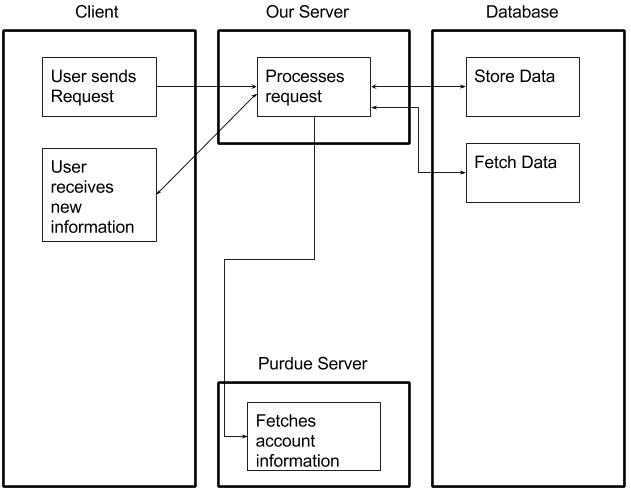
\includegraphics[width=.5\textwidth]{client-server-database}
\caption{High level overview diagram}
\end{figure}

Our application will use a client-server architecture: a user uses a client to send requests to our server, which may send queries to or fetch data from a database. The server then returns a response, which is parsed by the client.

\section{Design Issues}
\subsection*{Architecture}

\noindent
Option 1: \textbf{Client-Server Architecture} \\
Option 2: Unified Architecture

\br

Client-server architecture fits our needs because we need a central point to control the meeting schedule for many users. The client-server architecture also makes our code base more modular and allows for front-end and back-end capabilities. This architecture also enables us to take advantage of existing libraries that will help us design our software as a web application. A unified architecture is less modular, making it more difficult for us to collaborate. The code for a unified architecture application may also become messary

\newpage
\subsection*{Back-end framework}

\noindent
Option 1: \textbf{Node.js} \\
Option 2: Flask

\br

Node.js is an open-source Javascript platform designed for creating fast network applications. It is event-driven and has a non-blocking I/O model, great for handling a large number of requests. Since Node.js uses JavaScript, asynchronous operations and manipulation of JSON is easy and efficient. Node.js is a mature framework and has an enthusiastic community in addition to a huge number of open-source libraries.

Flask is used for quick prototyping of small projects: it is much more lightweight and has much fewer packages. As a microframework, it is designed for smaller projects with less complexity. For a feature-rich application like ours, Flask does not provide the same features or extensibility that comes with Node.js.

\subsection*{Front-end framework}

\noindent
Option 1: AngularJS \\
Option 2: \textbf{None (Pug templating engine for controller logic)}

\br

One of the most popular solutions for a front-end framework is AngularJS. By using AngularJS we would be committed to developing a model-view-controller (MVC) architecture. However, the major downside of AngularJS is its learning curve. We decided that it would take too long for our team to be properly acquainted with such a complex framework. Due to time constraints, we will initially avoid using a framework and opt for a less restricted way of implementing our front-end. In order to create some functionality that mimics a front-end framework, we will utilize the templating engine Pug. Using Pug, we will be able to quickly add conditional logic to our templates.

\subsection*{Database software}

\noindent
Option 1: MongoDB \\
Option 2: \textbf{MySQL}

\br

MongoDB is one of the most popular databases used in conjunction with Node.js. MongoDB stores objects in a JSON-like format, interfacing nicely with JSON queries sent from our Node.js server. This allows us to use a uniform language throughout our technology stack and manipulate database objects easily. However, as MongoDB is a document database, it is not suited for storing relationships between different objects, which is critical to our application.

The main selling point for MySQL, in terms of our project, is that it provides a relational-database for us to work with. Since our project has complex relationships (users, schedules, groups, etc.), it makes sense to minimize the number of database queries and simplify our application overall by using a relational database. We plan on using MySQL since it provides powerful relational queries that our application needs.

\subsection*{UX design}

\noindent
Option 1: Adaptive \\
Option 2: \textbf{Responsive}

\br

Responsive design and adaptive design both attempt to optimize the user experience. Responsive design is meant to be flexible: an example is a website that resizes and adjusts its UI for mobile devices. An adaptive design detects the settings of the device and then provides the appropriate layout. While both choices are feasible and provide a good user experiene, we have chosen to use a responsive design. A responsive design is effective and is easier to develop. Adaptive design is resource heavy and more difficult to implement.

\subsection*{Notification system}

\noindent
Option 1: Text \\
Option 2: \textbf{Email}

\br

Users can configure whether they want to receive notifications through email or through the messaging section of our application. There are several issues with text notifications: it requires additional user information, may potentially cost additional fees, and is generally less desirable than email notifications. Our notifications will be disabled by default to avoid undesirable spam: users who want to opt-in may do so after registering.

\section{Design Details}
\subsection*{Class Diagram}

\begin{figure}[H]
\centering
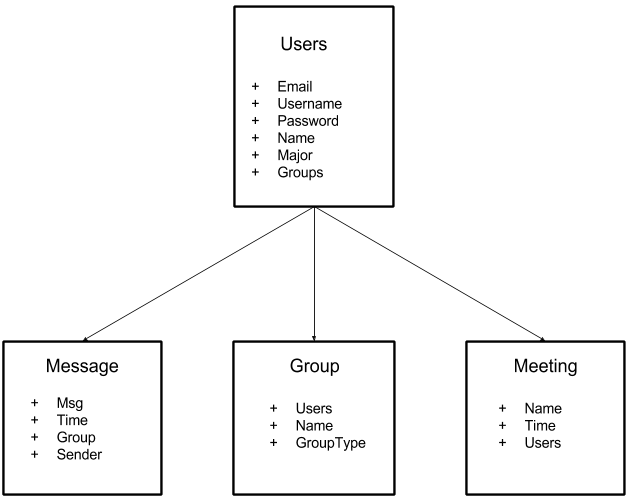
\includegraphics[width=.5\textwidth]{class-diagram}
\caption{Class Diagram}
\end{figure}

The User class represents users of our application. Users can form groups, send chat messages, and set meeting times. A User objects contains several fields: email, username, password, name, and major. The Group class represents a group of users. A Group object contains a group name, a collection of users, and a group type, which can be either be \code{group} (3 or more people) or a \code{private-message} (2 people). The Message class represents a chat message: it contains a message string, a timestamp, a group id, and a sender id.

\subsection*{Account Creation and User Login}

\begin{figure}[H]
\centering
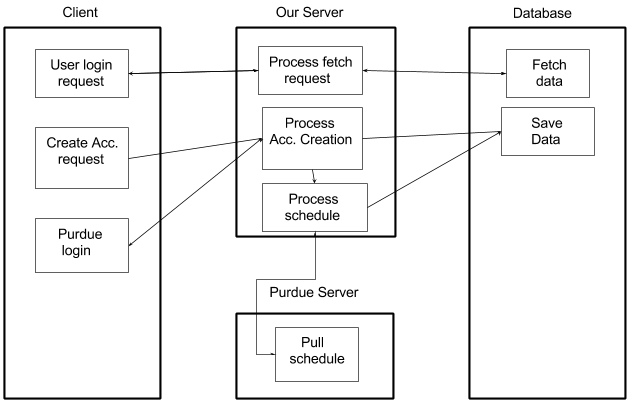
\includegraphics[width=.5\textwidth]{account-creation}
\caption{Account Creation and User Login}
\end{figure}

The user submits an account creation request to the server. The server then validates and processes the request, creating a user object and storing all relevant user information such as email, username, and a hashed password. The server then prompts the user for their Purdue Career account information if they would like to pull their schedule from the Purdue server. If accepted, the server then pulls the user's schedule from Purdue, and stores it in the database.

\subsection*{Token Authentication Process}

\begin{figure}[H]
\centering
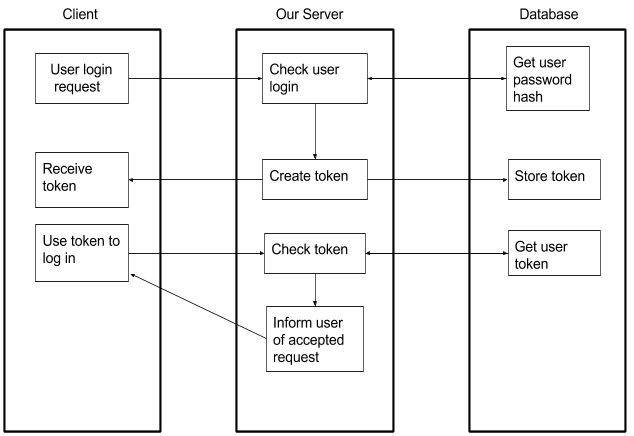
\includegraphics[width=.5\textwidth]{token_auth}
\caption{Authentication Process}
\end{figure}

The token authentication system starts when a user logs in with their credentials. The server then authenticates the user’s username and hashed password using information stored in the database. If the authentication succeeds, a session token will be stored in the database and sent to the user. This session token allows users to stay authenticated for a preset amount of time (for example, 7 days). While a user's session token remains valid and they have not logged out, they remain logged in and can perform any account-related actions.

\subsection*{Database Schema}

\begin{figure}[H]
\centering
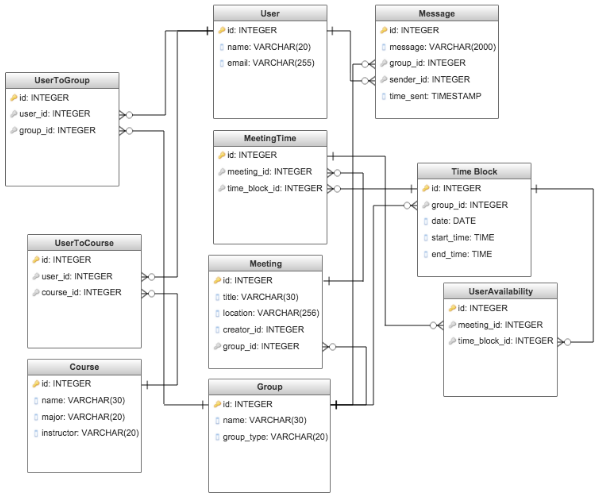
\includegraphics[width=.65\textwidth]{mysql-schema}
\caption{Database Schema}
\end{figure}

Our database schema for MySQL has 10 separate tables. Some of these tables contain foreign keys used for relational queries. Our database design utilizes One-To-Many and Many-To-Many relationships to store associations between \code{users$\leftrightarrow$groups}, \code{users$\leftrightarrow$courses}, \code{time blocks$\leftrightarrow$users}, and \code{time blocks$\leftrightarrow$meetings}.

Each table has a primary key: the \code{id} field. The \code{id} field is an auto-incrementing integer which represents a unique id for each row in a table.

The User table represents the User class: it stores properties such as users' name, email, major and any other user information and settings.

The Group table represents the Group class: it stores groups' names and their group type. The group type will be stored as a varchar in order to preserve readability in our database. There are two group types: \code{group} and \code{private-message}. In order to keep track of which groups users are in, we will create the UserToGroup table which contains foreign keys for \code{user-id} and \code{group-id}.

The Message table stores messages for all types of groups, it will include fields to keep track of the sender, the recipient group, the message text and the message timestamp.

The TimeBlock table is used to keep track of time ranges for possible times to hold a meeting. In order to allow a mapping between time blocks and users, we will create the UserAvailabilty table with foreign keys for \code{meeting-id} and \code{time-block-id}. Similarly, in order to mark which times are available for meetings we will have the MeetingTime table with foreign keys for \code{meeting-id} and \code{time-block-id}.

The Course table stores the list of courses that students are enrolled in, keeping track of specific properties such as the course department, instructor, and course title.

Finally, the UserToCourse table keeps track of the courses that users are enrolled in. This has foreign keys for \code{user-id} and \code{course-id}.

\subsection*{UI Mockups}

\begin{figure}[H]
\centering
\frame{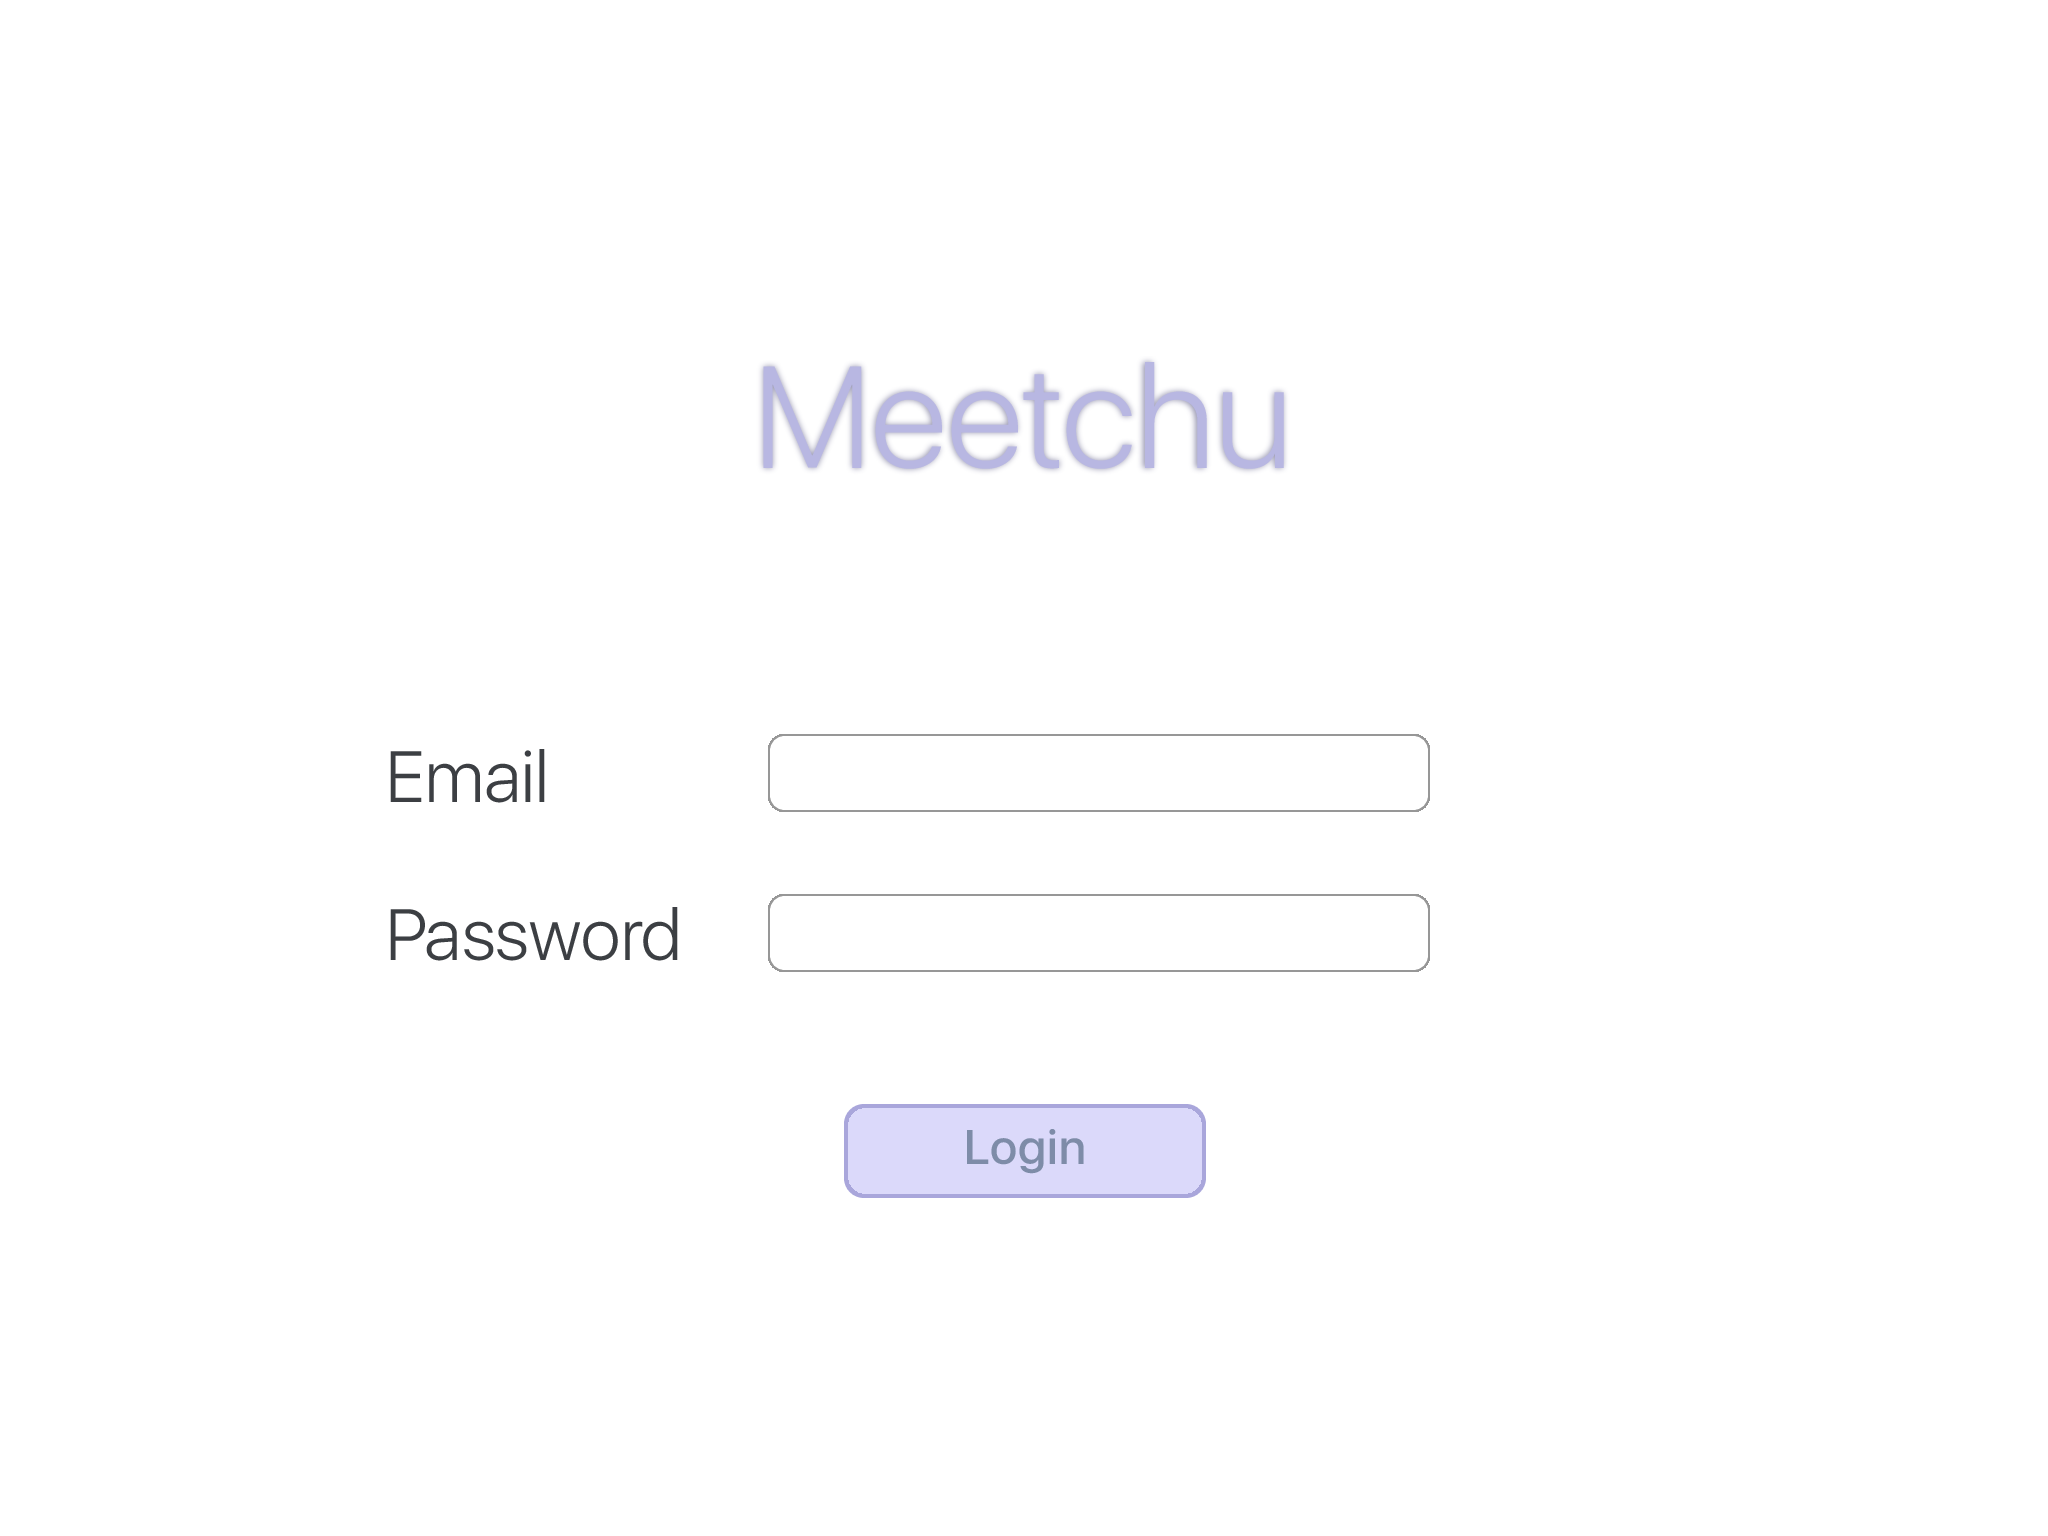
\includegraphics[width=.78\textwidth]{ui-login}}
\caption*{\footnotesize Desktop login page.}
\end{figure}

\begin{figure}[H]
\centering
\frame{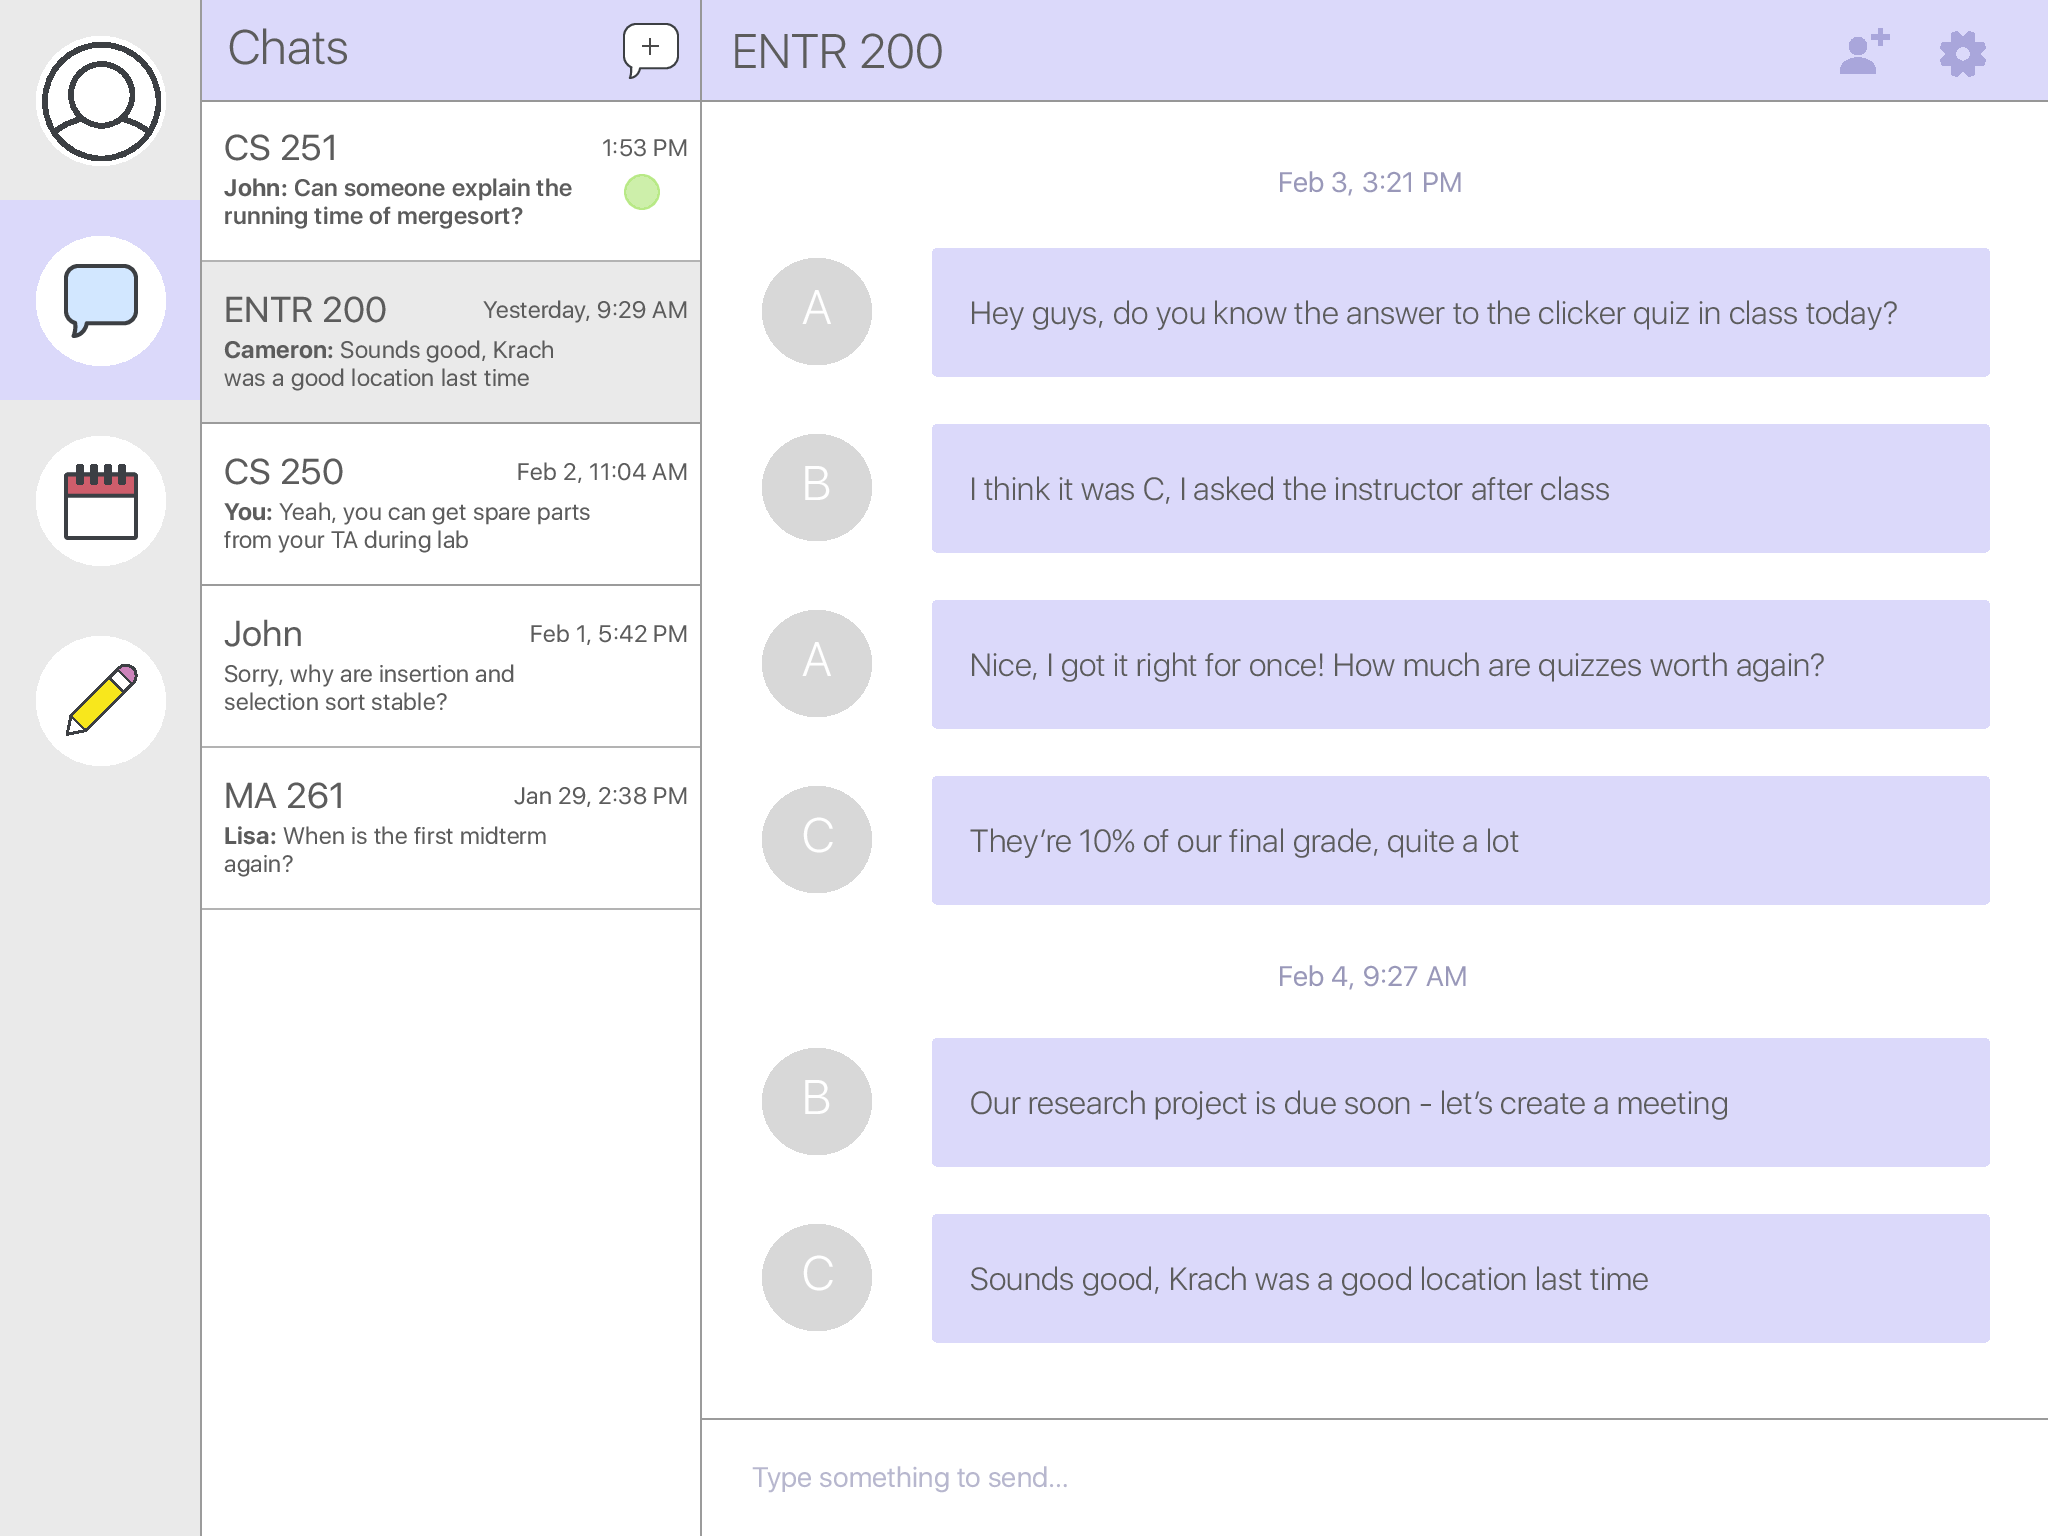
\includegraphics[width=.78\textwidth]{ui-chats}}
\caption*{\footnotesize Messaging page. It displays group and individual chats. Users can create new chats, add people to existing chats, and send messages.}
\end{figure}

\begin{figure}[H]
\centering
\frame{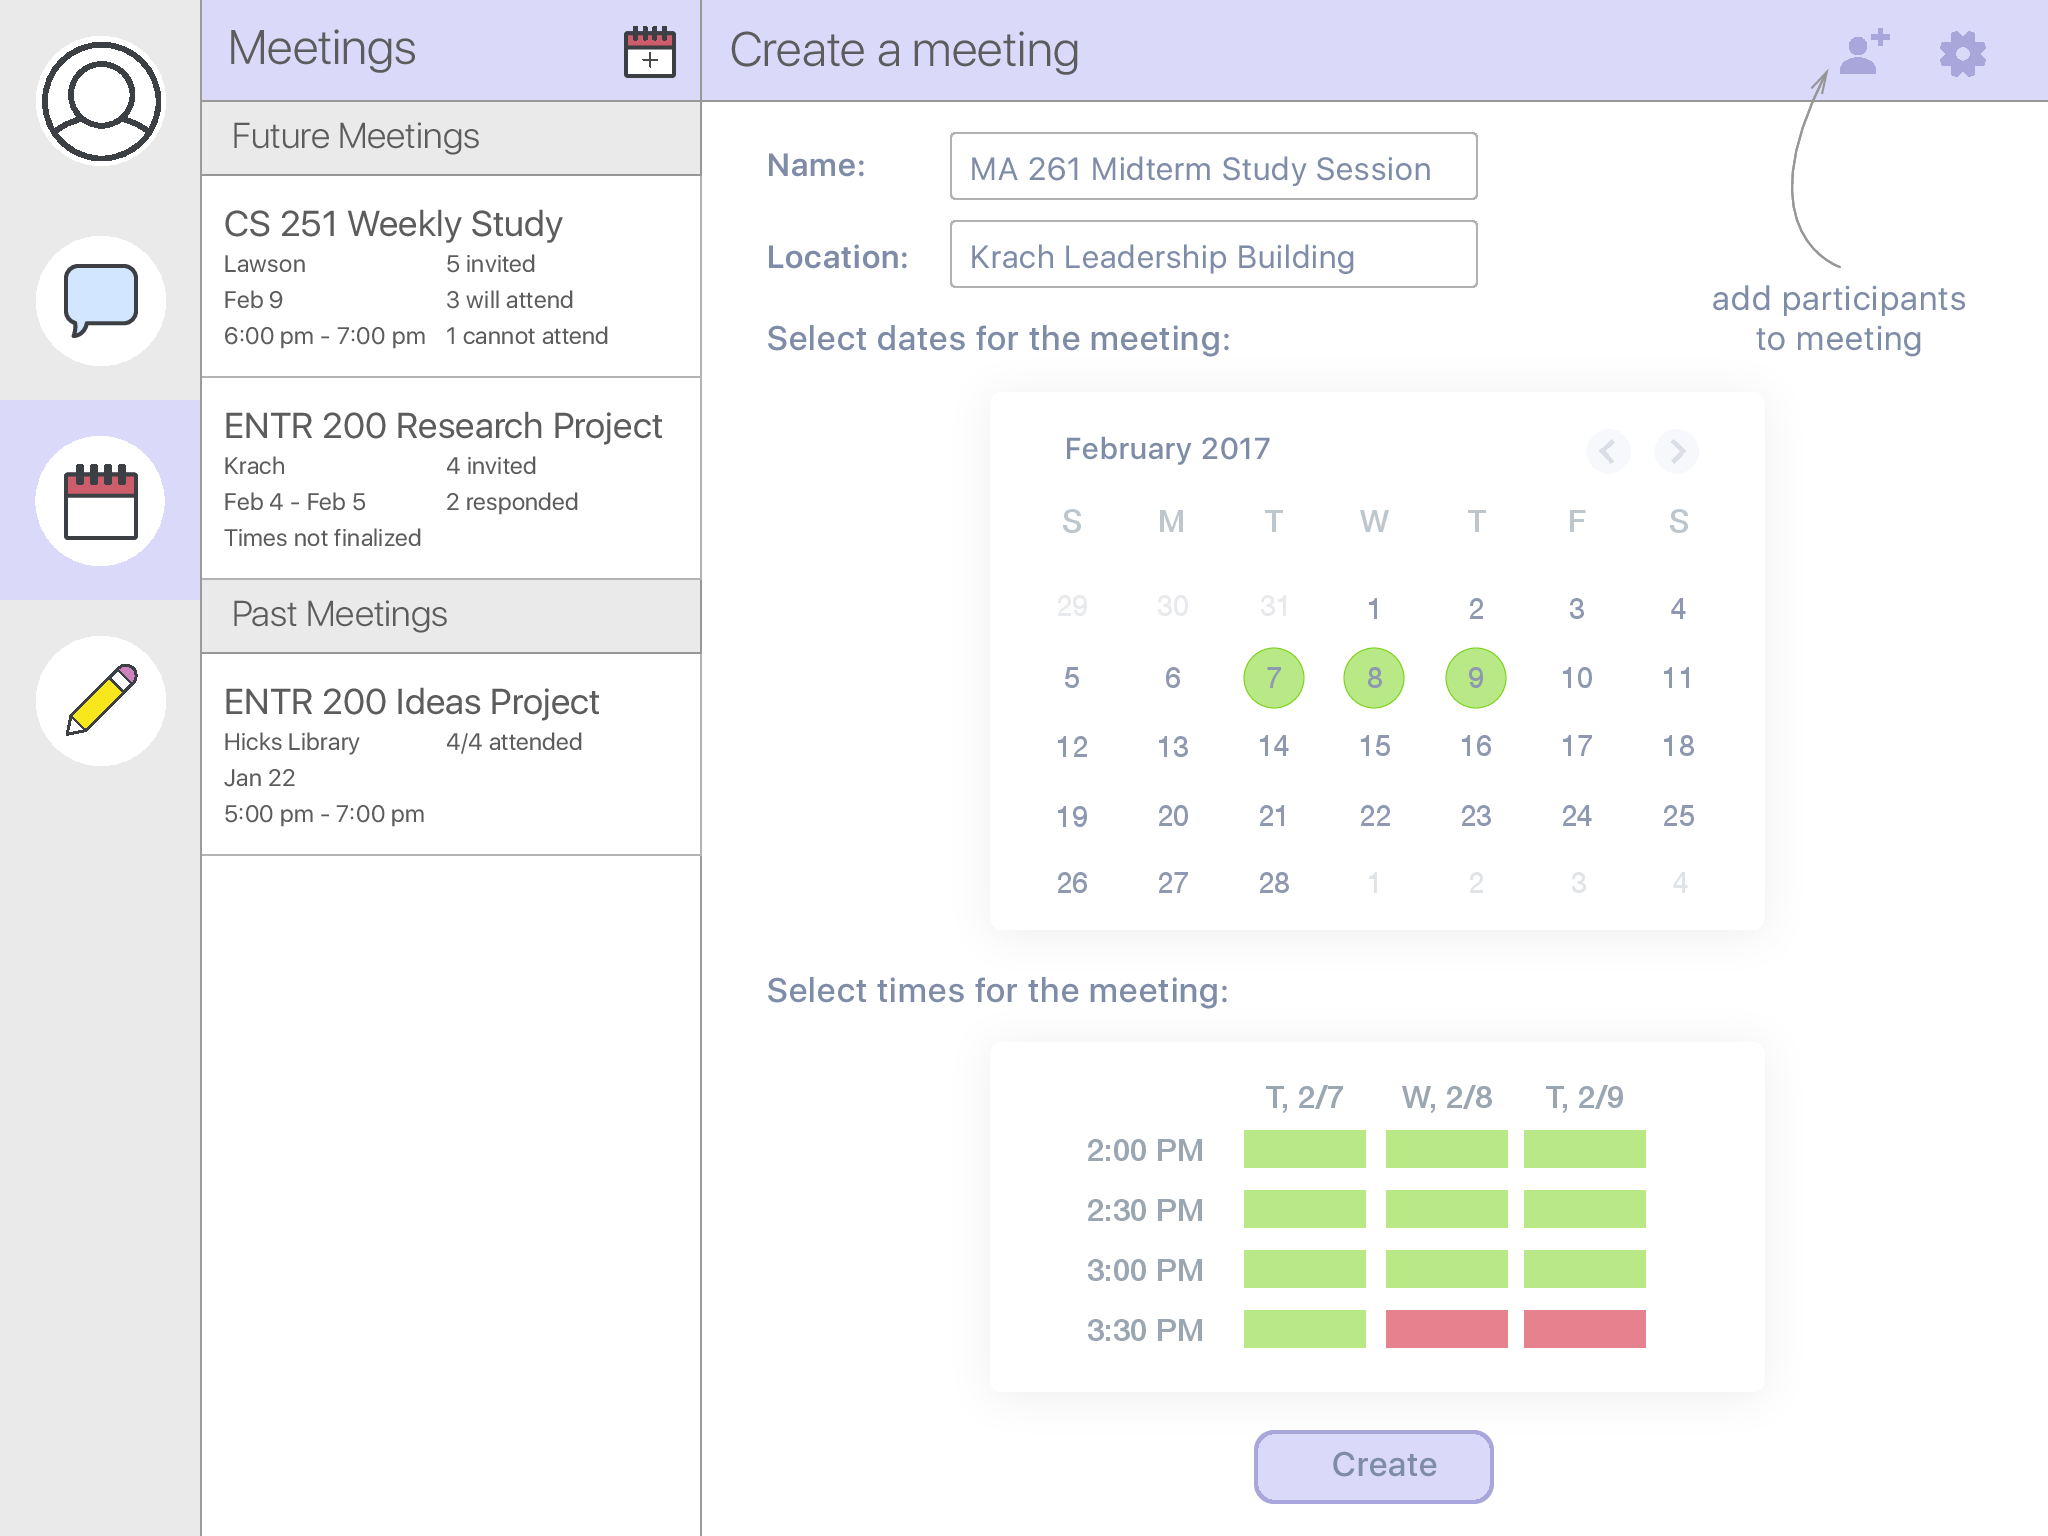
\includegraphics[width=.78\textwidth]{ui-meetings}}
\caption*{\footnotesize Meetings page. Users can create meetings, specify a name and location, propose meeting times, and add participates.}
\end{figure}

\end{document}
